\documentclass{article}
\documentclass{article}
\usepackage[utf8]{inputenc}
\usepackage{fullpage}
\usepackage{amsmath, mathtools}
\usepackage{amsfonts}
\usepackage{amssymb}
\usepackage{graphicx}
\usepackage{colortbl}
\usepackage{xr}
\usepackage{hyperref}
\usepackage{longtable}
\usepackage{xfrac}
\usepackage{tabularx}
\usepackage{float}
\usepackage{siunitx}
\usepackage{booktabs}
\usepackage{caption}
\usepackage{pdflscape}
\usepackage{afterpage}
\usepackage{seqsplit}
\usepackage{underscore}
\usepackage{lscape}
\usepackage[english]{babel}
\usepackage[T1]{fontenc}
\usepackage{booktabs}
\usepackage{tabularx}
\usepackage{hyperref}
\usepackage{nameref}

\hypersetup{
    colorlinks=true,       % false: boxed links; true: colored links
    linkcolor=red,          % color of internal links (change box color with linkbordercolor)
    citecolor=green,        % color of links to bibliography
    filecolor=magenta,      % color of file links
    urlcolor=cyan           % color of external links
}

%% Comments

\usepackage{color}

\newif\ifcomments\commentstrue %displays comments
%\newif\ifcomments\commentsfalse %so that comments do not display

\ifcomments
\newcommand{\authornote}[3]{\textcolor{#1}{[#3 ---#2]}}
\newcommand{\todo}[1]{\textcolor{red}{[TODO: #1]}}
\else
\newcommand{\authornote}[3]{}
\newcommand{\todo}[1]{}
\fi

\newcommand{\wss}[1]{\authornote{blue}{SS}{#1}} 
\newcommand{\plt}[1]{\authornote{magenta}{TPLT}{#1}} %For explanation of the template
\newcommand{\an}[1]{\authornote{cyan}{Author}{#1}}

%% Common Parts

\newcommand{\progname}{Mechatronics Engineering} % PUT YOUR PROGRAM NAME HERE
\newcommand{\authname}{Team \# 34, ParkingLotHawk
\\ Fady Zekry Hanna, zekryhf
\\ Winnie Trandinh, trandint
\\ Muhammad Ali, alim102
\\ Muhammad Khan, khanm120} % AUTHOR NAMES                  

\usepackage{hyperref}
    \hypersetup{colorlinks=true, linkcolor=blue, citecolor=blue, filecolor=blue,
                urlcolor=blue, unicode=false}
    \urlstyle{same}
                                


\title{Hazard Analysis\\\progname}

\author{\authname}

\date{}

\begin{document}

\maketitle
\thispagestyle{empty}

~\newpage

\pagenumbering{roman}

\begin{table}[hp]
\caption{Revision History} \label{TblRevisionHistory}
\begin{tabularx}{\textwidth}{llX}
\toprule
\toprule {\bf Date} & {\bf Version} & {\bf Notes}\\
\midrule
October 19, 2022 & 1.0 & Initial Revision \\
\bottomrule
\end{tabularx}
\end{table}

~\newpage

\tableofcontents

\listoftables

\listoffigures

~\newpage

\pagenumbering{arabic}

%%%%%%%% --------------------------------------------DOCUMENT START --------------------------------------------%%%%%%%%




%%%%%%%% --------------------------------------------INTRODUCTION --------------------------------------------%%%%%%%%



\section{Introduction}

Safety is a key feature of almost all products and services used. In order to determine safety features, a Hazard Analysis is typically done to generate, understand, and resolve key hazards that may come up during operations. For this document, a hazard is defined as a property or condition within the physical or virtual constraints of the system, together with a condition in the environment that has the potential to cause harm or damage. A Hazard Analysis of the ParkingLotHawk is presented in this document. 

%%%%%%%% --------------------------------------------Scope and Purpose of Hazard Analysis --------------------------------------------%%%%%%%%
\section{Scope and Purpose of Hazard Analysis}

The purpose of the Hazard Analysis is to find, understand and finalize resolutions to the various hazards that may occur.  

The product, ParkingLotHawk, is an Autonomous Aerial Drone used to gather live images and data within the confines of any given outdoor parking lot. The drone records the situation of each parking space periodically, and the information is sent to the user staying on the property in a timely manner. The user of such a product is the Parking Lot Operator (called Operator for short), who communicates with the Aerial Drone using an application running on their PC.

The scope of this Hazard Analysis is related to hazards that occur when the Parking Lot Operator is using the final product in the typical real-world use case: investigating an outdoor parking lot. For example, Hazards related to the development and prototyping of the product are not analyzed in this document. 

The document starts by breaking the system into components, followed by identifying hazards for each component using the Failure Modes and Effects Analysis (FMEA) method, and then finally generates new safety requirements to resolve the various hazards. This method will help minimize any unsafe behavior in the system by finding any possible causes of the said failure and determining the proper response for it.

%%%%%%%% --------------------------------------------System Boundaries and Components --------------------------------------------%%%%%%%%
\section{System Boundaries and Components}
\label{SystemBoundaries}
The systems referenced in this document for conducting ParkingLotHawk’s hazard analysis are defined within the \nameref{tab:SystemComp}:

\begin{table}[!h]
\begin{center}
\caption {System Components Table} 
\label{tab:SystemComp}
\begin{tabular}{ | m{4 cm} | m{12 cm} | } 
\hline
Components & Description \\
\hline
Main Drone Application & The Main Drone Application contains an implementation of the Finite State Machines specified in the Software Requirements Specification. This component also communicates with the Operator's PC Application to receive user commands and send relevant parking lot information.\\
\hline
Flight Operations & This component is responsible for calculating the optimal propeller speeds to stabilize and move the drone in accordance with movement commands from the Main Application. This component consists of the flight controller hardware, the external sensors it uses, and firmware that is flashed onto the flight controller board. Internal sensors include the Inertial Measurement Unit (IMU) for estimating acceleration and angular rate, a compass for orientation, and a barometer for atmospheric pressure to determine the altitude. External sensors include the Global Positioning System (GPS), used to locate the drone's position. \\
\hline
Vision Perception & The Vision Perception component consists of a camera and the algorithm for detecting parking spots, making an occupancy map of the lot, and segmenting the boundaries of the parking lot. It outputs segmentation, detections of parking lots, occupancy map, and live images that are used by the Main Drone Application. \\
\hline
Path Planner & This software component is used for autonomous exploration; it creates a path to explore the parking lot. Its outputs are used by the Main Drone Application. \\
\hline
Thrust Components & The Thrust Component is responsible for spinning the propellers at the speed commanded by the Flight Operations component. The component consists of motors, propellers, and Electronic Speed Controllers (ESCs).\\
\hline
Frame & The Frame will hold all the physical pieces of the drone together.\\
\hline
Power Modules & The Power Modules will power components within the drone such as the flight controller and motors. The components consist of a battery, charging equipment, switches, and wires.\\
\hline
Operator's PC Application & This component is what the Operator interfaces with to get the drone up and running, in addition to how the Operator obtains the information provided by the drone. This component communicates with the Main Application running on the physical drone to send user commands and receive relevant parking lot information. \\
\hline

\end{tabular}
\end{center}
\end{table}

\clearpage
Figure \ref{fig:SystemCompDiagram} below visualizes all of the system components within the project. 


\begin{figure}[!h]
    \centering
    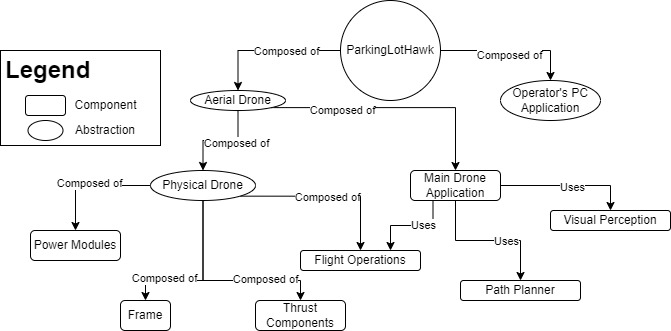
\includegraphics[width=1\textwidth]{HA/System Components.jpg}
    \caption{Systems Components Diagram}
    \label{fig:SystemCompDiagram}
\end{figure}


%%%%%%%% --------------------------------------------Critical Assumptions --------------------------------------------%%%%%%%%


\section{Critical Assumptions}
There are several assumptions that help to solve and sometimes even eliminate hazards all together. Firstly, it is assumed that the Parking Lot Operator utilizing the drone has completely read the User Manual and that they utilize the drone in the way specified by the User Manual. For example, if the User Manual specifies weather conditions under which the drone should not be flown, it is assumed that the user does not fly the drone in these inclement weather conditions. Secondly, it is assumed that the Operator uses the drone solely for parking lot investigation, not for activities such as recreation, spying, etc.  



%%%%%%%% --------------------------------------------Failure Mode and Effect Analysis --------------------------------------------%%%%%%%%
\section{Failure Mode and Effect Analysis}

The analysis of the components outlined within \nameref{SystemBoundaries} are provided through FMEA tables below, with the associated Safety Requirements attached to any applicable hazards.

\begin{landscape}
\begin{table}[!h]
\begin{center}
\caption {FMEA Table related to Flight Operation Components.} 
\label{tab:FMEA_Flight}
\begin{tabular}{ | m{1.2 cm} | m{2.8cm} | m{3cm} | m{1cm} | m{2.5 cm} | m{0.7cm} | m{0.6cm} | m{0.6cm} | m{3.5cm}| m{0.7cm} | m{0.5cm} | } 
\hline
 Design Component & Failure Mode & Effect of Failure & \seqsplit{Severity} & Causes of Failure & \seqsplit{Occurrence} & \seqsplit{Detection} & RPN & Recommended Action & SR & Ref \\
\hline
Flight Operation & IMU gives inaccurate readings. & The Drone is unable to determine angular orientation, which makes flight motion and stabilization difficult. & 10 &  IMU damaged during flight, magnetic interference.  & 2 & 7 & 140 &  Implement Flight Controller with secondary IMU, providing diversity and redundancy. & \nameref{SR_004} & H_001 \\
\hline
Flight Operation & Compass gives inaccurate readings. & Drone has difficulty in determining heading in space. & 7 & Compass damaged during flight, magnetic interference.  & 3 & 7 & 147 &  Implement Flight Controller with secondary compass, providing diversity and redundancy. & \nameref{SR_004} & H_002 \\
\hline
Flight Operation & Barometer gives an inaccurate reading. & Flight controller unable to determine altitude, creates difficulty in landing. & 9 & Barometer damaged during flight, UV/motor backwash interference.  & 2  & 7 & 126 &   Add an ultrasonic sensor at the bottom of the drone, providing a secondary height estimate. Although this only works for a short range (0-2m) it is sufficient for landing. & \nameref{SR_005} & H_003 \\
\hline
Flight Operation & Firmware unable to make the drone hover in place. Hovering was specified as stabilizing and staying within some tolerance of a location in space for a sufficiently long time. & Drone will not be able to fly to locations or follow paths well. Drone being unable to hover means that the camera will see blurry and shaky images. & 10 & Flight Controller internal malfunction, inclement weather (such as high winds).  & 1  & 2 & 20 &   Mention maximum wind requirement in User Manual. Report malfunction to Operator and enter the Malfunction state. & \nameref{SR_006}, \nameref{SR_007} & H_004 \\
\hline
Flight Operation & GPS Connection is lost or weak. & The drone will have a less accurate estimate of position, and thus won't be able to perform autonomous missions or move to a specific GPS locations.  & 10 & GPS damaged during flight, magnetic interference. & 3 & 7 & 210 &  Implement an alternative localization method via the camera or other range finder sensor, such as SLAM or optical flow.  & \nameref{SR_008} & H_005 \\
\hline
\end{tabular}
\end{center}
\end{table}
\end{landscape}

\begin{landscape}
\begin{table}[!h]
\begin{center}
\caption {FMEA Table related to Visual Perception.} 
\label{tab:FMEA_Vision}
\begin{tabular}{ | m{1.2 cm} | m{2.8cm} | m{3cm} | m{1cm} | m{2.5 cm} | m{0.7cm} | m{0.6cm} | m{0.6cm} | m{3.5cm}| m{0.7cm} | m{0.5cm} | }  
\hline
Design Component & Failure Mode & Effect of Failure & Severity & Causes of Failure & \seqsplit{Occurrence} & \seqsplit{Detection} & RPN & Recommended Action & SR & Ref \\
\hline
Visual Perception & Camera gives poor quality images or no image at all. & The primary functionality of showing the Operator the parking lot cannot be accomplished. Furthermore, the camera cannot detect the boundaries of the parking lot, causing the drone to be unable to perform autonomous tasks. & 8 & Camera lens is foggy or has other obstructions, or the camera is damaged during flight. & 3 & 1 & 24 &  Operator will detect the low image resolution themselves while they watch the live video. Operator may choose to wait or land the drone, clean the lens, restart the drone, and/or reconfigure it to fly closer to the ground.  & \nameref{SR_001} & H_006 \\
\hline
Visual Perception & Drone fails to detect the parking lot. & Drone is unable to implement autonomous states, and can only implement manual movement commands.  & 5 & Perception algorithm performs poorly due to weather conditions or the uniqueness of the parking lot. & 2 & 3 & 30 &  Operator should notice from the live camera images that the drone is consistently failing to correctly segment the parking lot, and thus the drone is only useful for true manual movement.  & \nameref{SR_006}, \nameref{SR_009} & H_007 \\
\hline
Visual Perception & Drone fails to detect the boundaries of the parking lot. & Drone is unable to implement autonomous states, and can only implement manual movement commands. During an autonomous state, the drone may exit the parking lot and not have noticed.  & 5 & Perception algorithm performs poorly due to weather conditions or the uniqueness of the parking lot.  & 4 & 3 & 60 &  Operator should notice from the live camera images that the drone is consistently failing to correctly segment the parking lot, and thus the drone is only useful for true manual movement.  & \nameref{SR_006}, \nameref{SR_009} & H_008 \\
\hline
\end{tabular}
\end{center}
\end{table}
\end{landscape}

\begin{landscape}
\begin{table}[!h]
\begin{center}
\caption {FMEA Table related to the Thrust Components and the Frame.} 
\label{tab:FMEA_Thrust}
\begin{tabular}{ | m{1.2 cm} | m{2.8cm} | m{3cm} | m{1cm} | m{2.5 cm} | m{0.7cm} | m{0.6cm} | m{0.6cm} | m{3.5cm}| m{0.7cm} | m{0.5cm} | }  
\hline
Design Component & Failure Mode & Effect of Failure & Severity & Causes of Failure & \seqsplit{Occurrence} & \seqsplit{Detection} & RPN & Recommended Action & SR & Ref \\
\hline
Thrust Components, Frame & An arm of the copter is unable to perform within its specifications, detected by the flight controller or noticed by the Operator. & The drone has fewer active propellers than it was tuned, trained, and designed for.  This will cause difficulty in flight and stabilization. & 8 & The given arm has a damaged propeller, damaged motor, broken electrical connection between the motor and ESC, mechanical disconnection between the propeller and motor, or a crack on the arm to the extent of not being able to provide a rigid frame. & 4 & 5 & 160 &  Although flight will be hindered, the firmware has the capabilities to still fly the drone under most conditions. The drone shall enter the malfunction state, trying to land at its original location. The Operator, being from a non-technical background, will need to send the drone for repair once recovered. In the user manual, it should be specified that the Operator is required to inspect the drone for damage prior to flight.  & \nameref{SR_002}, \nameref{SR_007} & H_009 \\
\hline
\end{tabular}
\end{center}
\end{table}
\end{landscape}

\begin{landscape}
\begin{table}[!h]
\begin{center}
\caption {FMEA Table related to the Frame.} 
\label{tab:FMEA_Frame}
\begin{tabular}{ | m{1.2 cm} | m{2.8cm} | m{3cm} | m{1cm} | m{2.5 cm} | m{0.7cm} | m{0.6cm} | m{0.6cm} | m{3.5cm}| m{0.7cm} | m{0.5cm} | }  
\hline
Design Component & Failure Mode & Effect of Failure & Severity & Causes of Failure & \seqsplit{Occurrence} & \seqsplit{Detection} & RPN & Recommended Action & SR & Ref \\
\hline
Frame & Center of frame cracked, as seen by Operator. &  Drone will have difficulty in flight. Parts of the drone may fall out if the crack is large enough. & 5 & Center of frame damaged during flight or storage. & 2 & 7 & 70 &  Enclose the central base of the drone such that components do not fall out. In the user manual, specify that the Operator is required to inspect the drone for damage prior to flight. If the Operator sees any cracks during flight, they should send the drone into the malfunction state. & \nameref{SR_001}, \nameref{SR_002}  & H_010 \\
\hline
Frame & Drone is very hot. &  Operator may be hurt if they touch the hot components. Drone components may also be damaged after prolonged heat exposure. & 5 & Overheating components due to component malfunction. & 5 & 7 & 175 &  Add heat sinks on electrical components and specify the correct way to hold the drone in the user manual. Also specify how long  the Operator must wait and let the drone cool down before making any contact with it. & \nameref{SR_010} & H_011 \\
\hline
\end{tabular}
\end{center}
\end{table}
\end{landscape}

\begin{landscape}
\begin{table}[!h]
\begin{center}
\caption {FMEA Table related to the Power Modules.} 
\label{tab:FMEA_Power}
\begin{tabular}{ | m{1.2 cm} | m{2.8cm} | m{3cm} | m{1cm} | m{2.5 cm} | m{0.7cm} | m{0.6cm} | m{0.6cm} | m{3.5cm}| m{0.7cm} | m{0.5cm} | }  
\hline
Design Component & Failure Mode & Effect of Failure & Severity & Causes of Failure & \seqsplit{Occurrence} & \seqsplit{Detection} & RPN & Recommended Action & SR & Ref \\
\hline
Power Modules & Low Battery. &  Drone will be unable to fly for a long duration of time. If Drone is not landed soon, it could run out of power mid-air and crash.  & 8 & Drone has been flying for a long duration, or recharge is not completed before use.  & 7 & 4 & 224 &  Once the drone detects less than 3 minutes of battery remaining, it shall automatically land the drone at it's original launch location and inform the Operator. & \nameref{SR_003}, \nameref{SR_011} & H_012 \\
\hline
Power Modules & Battery capacity low. &  Drone will be unable to fly long enough to complete its functions. & 8 & Drone's battery life has deteriorated over time.  & 2 & 6 & 96 &  Drone should prevent flight if the battery capacity is less than 3 minutes, and the drone should convey to the Operator that it cannot fly and state the reason why. The Operator will need to purchase a new battery replacement.  & \nameref{SR_003}, \nameref{SR_012} & H_013 \\
\hline
Power Modules & Wire connections become loose. &  Electrical components  and system will not function correctly. & 9 & Wires may become loose after extended use or upon damage. & 2 & 7 & 126 &  Solder all electrical wires and attach heat shrinks or crimps to wire-to-wire connections.  & - & H_014 \\
\hline
Power Modules & Drone smokes or ignites. &  Drone is unable to function properly and the safety of the Operator is diminished. & 10 & Wires is short circuited due to damage, motors are damaged, or the battery is damaged or punctured. & 2 & 2 & 40 & Require the Operator to perform a visual inspection before flight, and ensure that the Operator has access to a Class B fire extinguisher.  & \nameref{SR_002} & H_015 \\
\hline
\end{tabular}
\end{center}
\end{table}
\end{landscape}

\begin{landscape}
\begin{table}[!h]
\begin{center}
\caption {FMEA Table related to the Operator's PC Application.} 
\label{tab:FMEA_OpApp}
\begin{tabular}{ | m{1.2 cm} | m{2.8cm} | m{3cm} | m{1cm} | m{2.5 cm} | m{0.7cm} | m{0.6cm} | m{0.6cm} | m{3.5cm}| m{0.7cm} | m{0.5cm} | }  
\hline
Design Component & Failure Mode & Effect of Failure & Severity & Causes of Failure & \seqsplit{Occurrence} & \seqsplit{Detection} & RPN & Recommended Action & SR & Ref \\
\hline
\seqsplit{Operator's} PC Application & Malicious user hacks into the Operator's PC Application via login system. &  Malicious users will be able to inspect the parking lot.  & 3 & Too simple of a login password or password leaked out.  & 1 & 10 & 30 &  Require that the passwords be sufficiently complicated: at least one upper case, one lower case, one number, and one special character. Also, denote in the user manual that the password should be kept a secret from external parties. & \nameref{SR_013} & H_016 \\
\hline
\end{tabular}
\end{center}
\end{table}
\end{landscape}

\begin{landscape}
\begin{table}[!h]
\begin{center}
\caption {FMEA Table related to the Path Planner.} 
\label{tab:FMEA_OpApp}
\begin{tabular}{ | m{1.4 cm} | m{2.8cm} | m{3cm} | m{1cm} | m{2.5 cm} | m{0.7cm} | m{0.6cm} | m{0.6cm} | m{3.5cm}| m{0.5cm} | m{0.5cm} | }  
\hline
Design Component & Failure Mode & Effect of Failure & Severity & Causes of Failure & \seqsplit{Occurrence} & \seqsplit{Detection} & RPN & Recommended Action & SR & Ref \\
\hline
Path Planner (also called Autonomous Explore) & Internal explore strategy malfunctions. The Operator notices the drone is not exploring the parking lot correctly. &  Drone may keep exploring the same area thus wasting time, or the drone may exit the parking lot.  & 4 & Due to the path planning algorithm not performing accurately/correctly. For faulty vision input, see \nameref{tab:FMEA_Vision}  & 4 & 8 & 128 &  It is upon the Operator to notice the inaccuracy of the path planning feature during the Autonomous Explore State, At which point the Operator should utilize other more accurate features instead (such as Manual Explore). & - & H_017 \\
\hline
\end{tabular}
\end{center}
\end{table}
\end{landscape}

\begin{landscape}
\begin{table}[!h]
\begin{center}
\caption {FMEA Table related to the Operator's PC Application and the Main Drone Application.} 
\label{tab:FMEA_MainApp_OpApp}
\begin{tabular}{ | m{1.2 cm} | m{2.8cm} | m{3cm} | m{1cm} | m{2.5 cm} | m{0.7cm} | m{0.6cm} | m{0.6cm} | m{3.5cm}| m{0.7cm} | m{0.5cm} | }  
\hline
Design Component & Failure Mode & Effect of Failure & Severity & Causes of Failure & \seqsplit{Occurrence} & \seqsplit{Detection} & RPN & Recommended Action & SR & Ref \\
\hline
\seqsplit{Operator's} PC Application, Main Drone Application & Drone loses connection to Operator's PC Application, or connection has deteriorated. For example, the connection has been lost for sufficiently long, the connection is very slow, weak, and/or delayed. &  Drone is unable to communicate to the Operator. The drone is unable to send its data to the Operator. The drone may also miss commands from the Operator.  & 10 & The connection is poor due to weather, distance, or network interference (such as another similar radio frequency in the nearby area). Another possible cause is the Operator's PC Application crashing.  & 6 & 1 & 60 &  Upon sufficiently poor connection detected for a sufficiently long time, the drone shall enter the Weak Connection State and convey this to the user if possible. In this state, the drone flies back to its original launch location, and if during flight it regains a sufficiently good connection for a sufficiently long time it resumes normal operation. & \nameref{SR_006}, \nameref{SR_007} & H_018 \\
\hline
\end{tabular}
\end{center}
\end{table}
\end{landscape}


\section{Safety and Security Requirements}
Multiple new requirements were discovered through the generation of the FMEA table. Each requirement is referenced with the hazard that revealed it in the FMEA tables above.

\begin{table}[!h]
\begin{center}
\caption {SR\_001} 
\label{SR_001}
\begin{tabular}{ | m{3cm} | m{11cm} | }
\hline
Description & The product shall include a user-controlled button that sends the product to a Malfunction state.
 \\
\hline
Rationale & The requirement ensures that the Operator can send the product into a Malfunction state if the Operator detects something wrong with the product. \\
\hline
Associated Hazard & H\_006, H\_010 \\
\hline
\end{tabular}
\end{center}
\end{table}

\begin{table}[!h]
\begin{center}
\caption {SR\_002} 
\label{SR_002}
\begin{tabular}{ | m{3cm} | m{11cm} | }
\hline
Description & The product shall inform the user that a visual inspection for damages is required before each use, such as through a user manual.
 \\
\hline
Rationale & The requirement ensures that the Operator is instructed to inspect the product before use for any damages that may impact its performance. \\
\hline
Associated Hazard & H\_009, H\_010, H\_015 \\
\hline
\end{tabular}
\end{center}
\end{table}

\begin{table}[!h]
\begin{center}
\caption {SR\_003} 
\label{SR_003}
\begin{tabular}{ | m{3cm} | m{11cm} | }
\hline
Description & The product shall provide a visual display of its estimated remaining battery life in minutes.
 \\
\hline
Rationale & The requirement ensures that the Operator is informed of the expected duration of operation remaining, such that the Operator can plan its operation accordingly. \\
\hline
Associated Hazard & H\_012, H\_013 \\
\hline
\end{tabular}
\end{center}
\end{table}

\begin{table}[!h]
\begin{center}
\caption {SR\_004} 
\label{SR_004}
\begin{tabular}{ | m{3cm} | m{11cm} | }
\hline
Description & The product shall feature redundant sensors that can be used for localization.
 \\
\hline
Rationale & The requirement ensures that the product can still function within its specifications even if its primary localization sensors such as the IMU are malfunctioning. \\
\hline
Associated Hazard & H\_001, H\_002 \\
\hline
\end{tabular}
\end{center}
\end{table}

\begin{table}[!h]
\begin{center}
\caption {SR\_005} 
\label{SR_005}
\begin{tabular}{ | m{3cm} | m{11cm} | }
\hline
Description & The product shall have a redundant method of determining its height.
 \\
\hline
Rationale & The requirement ensures that the product can safely land in the event that the primary method of height determination is malfunctioning. \\
\hline
Associated Hazard & H\_003 \\
\hline
\end{tabular}
\end{center}
\end{table}

\begin{table}[!h]
\begin{center}
\caption {SR\_006} 
\label{SR_006}
\begin{tabular}{ | m{3cm} | m{11cm} | }
\hline
Description & The product shall inform the user of the environmental conditions where the product cannot be used, such as through the user manual. \\
\hline
Rationale & The requirement ensures that the Operator does not use the product within inclement weather, as the product is not designed to operate in such conditions. \\
\hline
Associated Hazard & H\_004, H\_007, H\_008, H\_017 \\
\hline
\end{tabular}
\end{center}
\end{table}

\begin{table}[!h]
\begin{center}
\caption {SR\_007} 
\label{SR_007}
\begin{tabular}{ | m{3cm} | m{11cm} | }
\hline
Description & Upon entering into the Malfunction States, the product shall inform the Operator through the Operator's application if the product and application can successfully communicate. \\
\hline
Rationale & The requirement ensures that the Operator is aware that the product has detected a malfunction, and that it has entered the malfunction state as opposed to continuing with its normal operation. \\
\hline
Associated Hazard & H\_004, H\_009, H\_017 \\
\hline
\end{tabular}
\end{center}
\end{table}

\begin{table}[!h]
\begin{center}
\caption {SR\_008} 
\label{SR_008}
\begin{tabular}{ | m{3cm} | m{11cm} | }
\hline
Description & The product shall have a secondary localization method that can be used when the GPS is non-functional. \\
\hline
Rationale & The requirement ensures that the product is still able to operate within its specifications in the event that its GPS sensor is malfunctioning. \\
\hline
Associated Hazard & H\_005 \\
\hline
\end{tabular}
\end{center}
\end{table}

\begin{table}[!h]
\begin{center}
\caption {SR\_009} 
\label{SR_009}
\begin{tabular}{ | m{3cm} | m{11cm} | }
\hline
Description & The product shall display a segmented image of the parking lot vs non-parking lot to the Operator's application. \\
\hline
Rationale & The requirement ensures that the Operator is aware of how the product is perceiving its environment, and can determine if the product's perception of its environment is correct or incorrect. \\
\hline
Associated Hazard & H\_007, H\_008 \\
\hline
\end{tabular}
\end{center}
\end{table}

\begin{table}[!h]
\begin{center}
\caption {SR\_010} 
\label{SR_010}
\begin{tabular}{ | m{3cm} | m{11cm} | }
\hline
Description & The product shall inform the user of how to hold the product, such as through the user manual. \\
\hline
Rationale & The requirement ensures that the product is not damaged by incorrect handling, nor is the Operator harmed by the product as a result of incorrect handling. \\
\hline
Associated Hazard & H\_011 \\
\hline
\end{tabular}
\end{center}
\end{table}

\begin{table}[!h]
\begin{center}
\caption {SR\_011} 
\label{SR_011}
\begin{tabular}{ | m{3cm} | m{11cm} | }
\hline
Description & The product shall automatically return to its original launch location and land once the estimated battery time is less than 3 minutes. \\
\hline
Rationale & The requirement ensures that the product has sufficient battery left to safely return to its landing area and land, all while remaining within its specifications. \\
\hline
Associated Hazard & H\_012 \\
\hline
\end{tabular}
\end{center}
\end{table}

\begin{table}[!h]
\begin{center}
\caption {SR\_012} 
\label{SR_012}
\begin{tabular}{ | m{3cm} | m{11cm} | }
\hline
Description & The product shall inform the user if the battery capacity before launch is estimated to be less than 3 minutes of flight, and prevent launch of the product. \\
\hline
Rationale & The requirement ensures that the product is not used with excessively worn out batteries, to the extent that it cannot operate within its specifications. \\
\hline
Associated Hazard & H\_013 \\
\hline
\end{tabular}
\end{center}
\end{table}

\begin{table}[!h]
\begin{center}
\caption {SR\_013} 
\label{SR_013}
\begin{tabular}{ | m{3cm} | m{11cm} | }
\hline
Description & The Operator's login password shall be sufficiently complex: shall feature at least one upper case, one lower case, one number, and one special number. \\
\hline
Rationale & The requirement ensures that the Operator's application is safe against malicious users. \\
\hline
Associated Hazard & H\_015 \\
\hline
\end{tabular}
\end{center}
\end{table}

\clearpage

\section{Roadmap}

The safety requirements will be implemented through 4 main phases, and are as follows:
\begin{itemize}
    \item Phase I: Proof of Concept - November 14, 2022
    \item Phase II: Revision 0 (Minimal Viable Product (MVP) ) - February 6, 2023 
    \item Phase III: Revision 1 - March 27, 2023
    \item Phase IV: Revision 2 - April 27, 2023
\end{itemize}

The requirements will be implemented within the respective phase as listed in Table \ref{SR_Roadmap}.

\begin{table}[!h]
\begin{center}
\caption {Safety Requirements Roadmap}
\label{SR_Roadmap}
\begin{tabular}{ | m{3cm} | m{11cm} | }
\hline
Phase I & \nameref{SR_002}, \nameref{SR_010} \\
\hline
Phase II & \nameref{SR_001}, \nameref{SR_006}, \nameref{SR_007}, \nameref{SR_013} \\
\hline
Phase III & \nameref{SR_003}, \nameref{SR_009}, \nameref{SR_011}, \nameref{SR_012} \\
\hline
Phase IV & \nameref{SR_004}, \nameref{SR_005}, \nameref{SR_008} \\
\hline
\end{tabular}
\end{center}
\end{table}


\end{document}